\documentclass[a4paper,12pt]{report}
\usepackage{amsmath,amssymb,amsthm,IEEEtrantools,hyperref,esint,multicol}
\usepackage{tikz,pgf,fancyhdr,pgfplots,lmodern,transparent}
\usepackage{float, graphicx, physics, titling, cite, bm}
\usepackage{array,multirow,textgreek}
\usepackage[justification=centering]{caption}
\usepackage[export]{adjustbox}
\usepackage[nopostdot, nonumberlist, nogroupskip, toc, automake]{glossaries}
\usepackage[nottoc]{tocbibind}
\usepackage[includeheadfoot, left=1.2cm, right=1.2cm, bottom=3cm, top=3cm]{geometry}

\hypersetup{
    colorlinks=true,
    linkcolor=blue,
    filecolor=green,      
    urlcolor=violet,
}

\pgfplotsset{width=10cm,compat=1.9}

\pagestyle{fancy}
\fancyhf{}
\rhead{Bachelor Thesis}
\cfoot{\thepage}
\lfoot{\includegraphics[scale=0.02,valign=c]{logo/USTH_logo.png}}
\rfoot{\includegraphics[scale=0.1,valign=c]{logo/SA_logo.png}}

\renewcommand{\headrulewidth}{1pt}
\renewcommand{\footrulewidth}{1pt}
\addtolength{\footskip}{0.5cm}
\setlength{\headheight}{15pt}
\newcommand{\la}{\left\langle}
\newcommand{\ra}{\right\rangle}
\newcommand{\pvec}[1]{\vec{#1}\mkern2mu\vphantom{#1}}
\theoremstyle{plain}\newtheorem{ques}{Question}
\theoremstyle{definition}\newtheorem*{ans}{Answer}

\author{Nguyen Hoang Dang Khoa}
\title{Mean-field study of the equation of states of nuclear matter and tidal deformation of neutron star}
\date{\today}

\makeglossaries
\newglossaryentry{NS}{name={NS}, description={Neutron Star}}
\newglossaryentry{NM}{name={NM}, description={Nuclear Matter}}
\newglossaryentry{EoS}{name={EoS}, description={Equation of States}}
\newglossaryentry{TOV}{name={TOV}, description={Tolmann-Oppenheimer-Volkoff}}
\newglossaryentry{HF}{name={HF}, description={Hartree-Fock}}
\newglossaryentry{GR}{name={GR}, description={General Relativity}}
\newglossaryentry{GE}{name={GE}, description={Gravito-electric}}
\newglossaryentry{GM}{name={GM}, description={Gravito-magnetic}}
\newglossaryentry{NN}{name={NN}, description={Nucleon-Nucleon}}

\newcolumntype{C}{>{$}c<{$}}

\begin{document}
        \begin{titlepage}
                \centering
                \newgeometry{top=1cm, bottom=2cm, left=2.5cm, right=2.5cm}
                {\transparent{0.9}\includegraphics[scale=0.08,valign=c]{logo/USTH_logo.png}\par}
                \vspace{0.3cm}
                {\scshape\Large University of Science and Technology of Hanoi \par}
                \vspace{6.3cm}
                \rule[-9pt]{\textwidth}{0.7pt}\par
                \rule{\textwidth}{1.6pt}\par
                \vspace{0.3cm}
                {\Huge\bfseries \thetitle\par}
                \vspace{0.2cm}
                {\Large\bfseries Bachelor Thesis\par}
                \vspace{0.3cm}
                \rule{\textwidth}{1.6pt}\par
                \rule[10pt]{\textwidth}{0.7pt}\par
                \vspace{0.5cm}
                % {\Large \theauthor\par}
                \begin{minipage}[t]{0.45\textwidth}
                        \begin{flushleft}
                                \emph{Author:}\\
                                Nguyen Hoang Dang \textsc{Khoa}
                        \end{flushleft}
                \end{minipage}
                \begin{minipage}[t]{0.3\textwidth}
                        \begin{flushright}
                                \emph{Supervisors:}\\
                                Prof. Dao Tien \textsc{Khoa}\\
                                Dr. Ngo Hai \textsc{Tan}
                        \end{flushright}
                \end{minipage}
                % \vspace{0.2cm}
                % {\large\bfseries BI9-128\par}
                \vfill
                {\large \thedate\par}
        \end{titlepage}  
        
        \restoregeometry
        \tableofcontents

        \printglossary[title={List of Abbreviations}]

        \chapter{Introduction}
        % \section{Neutron Stars and Nuclear Matter}%
% \label{sec:neutron_stars_and_nuclear_matter}

Neutron stars (\gls{NS}) are the compact astronomical objects known also as pulsars, 
formed shortly after the core-collapse supernova as a super dense, giant liquid drop 
of strongly interacting baryons and leptons. With the NS gravitational mass $M$ up to 
twice the solar mass $M_\odot$, NS matter is enclosed tightly within a radius of 
$R\sim 10-12$ km and the baryon density $n_b$ inside the NS core is several times 
larger than the normal matter density in center of a heavy nucleus like 
$^{208}$Pb ($n_0 \approx 0.17$ fm$^{-3}$). 
Neutron stars are in fact the densest accessible astronomical objects in the Universe 
after black holes \citep{baym1975neutron}, and the physics effects by all the four 
fundamental interactions have been found from the astrophysical observations 
of the single- and binary pulsars. Therefore, NS is an ideal natural ``laboratory'' 
for the modern physics research that links different fields of physics, like atomic
and nuclear physics, high-energy physics, and astrophysics \citep{lattimer2004physics}.

The massive neutrino emission during the cooling of hot proto-neutron star (\gls{PNS}) formed 
instantly after supernova proceeds mainly via the weak process of electron capture 
by protons in the PNS core   
\begin{equation}
        p + e^- \to n + \nu_e,
\end{equation}
leading to a huge excess of neutrons in the core, and hence the name ``neutron star''.
In fact, neutrons in the dense core of NS are not bound by the strong force between baryons 
but they are packed tightly by a hydrostatic balance between the pressure of NS matter
and gravitation. In this study, we focus on cold \gls{NS} after a considerable time 
from its formation, when the temperature is considered to be $T=0$.

Below the atmospheric gas layer of \gls{NS}, the low-density matter of NS \emph{crust}
is highly inhomogeneous. With the increasing density, the NS matter gradually becomes more 
or less uniform so that the dense core of NS can be treated as an uniform, neutron-rich
nuclear matter (NM) which is referred to hereafter as asymmetric NM (see illustration in  
Figure \ref{fig:NS_structure}). It is obvious that one needs to use a proper nuclear physics
model to determine the pressure of fully degenerated baryons and that of leptons in NS matter 
at different matter densities in order to determine the macroscopic properties of NS 
within the frame of General Relativity (GR). Over the years, different nuclear mean-field 
models have been used to construct the \emph{equation of states} (\gls{EoS}) of asymmetric NM, 
which gives the behavior of macroscopic properties of NM like the pressure $P$ and mass-energy 
density $\varepsilon$ with the increasing NM density. Among these studies, the nonrelativistic
Hartree-Fock (\gls{HF}) approach to study NM using an appropriate effective (in-medium) 
nucleon-nucleon (NN) interaction has been well proven to give a realistic description 
of asymmetric NM up to very high baryon densities \citep{khoa1996study}. Because the NN 
interaction in a dense medium of NM is very different from the free NN interaction, the use 
of an effective density dependent NN interaction is widely adopted in the mean-field 
calculations of NM, although
some ab-initio many-body calculations of NM using the QCD-based interaction between baryons
are now feasible with the supercomputer of very high performance. In the present work, we
perform the HF calculation of asymmetric NM using the well-tested CDM3Yn model of the effective
density dependent NN interaction \citep{tan2021equation}, which is presented in details
in Section \ref{chap:hf}. A rapidly rotating NS or pulsar is known to have a strong intrinsic
magnetic field, and significant fractions of protons and neutrons in NS matter might  
have their spins polarized along the axis of magnetic field \cite{broderick2000equation}. To explore the effects
by the spin polarization of baryons, we have extended the conventional HF method to the calculation
of the EoS of spin-polarized NM. which is further used to generate NS matter that consists 
of strongly interacting baryons (protons and neutrons) and leptons (electrons and muons) 
being in \textbeta-equilibrium. The EoS of the inhomogeneous crust of NS taken from the 
compressible liquid drop model \citep{douchin2000nuclear,douchin2001unified} is added to the \gls{EoS} of the \textbeta-stable 
NS matter given by the present \gls{HF} calculation, to obtain the full input
for NS matter. Such a mean-field input of the EoS of NS matter can then be used in GR 
to determine the gravitational mass and radius of NS \citep{tan2020spin,tan2021equation} 
from the solution of the Tolman-Oppenheimer-Volkoff (\gls{TOV}) equations \citep{oppenheimer1939massive}. 

\begin{figure}[t]
        \centering
        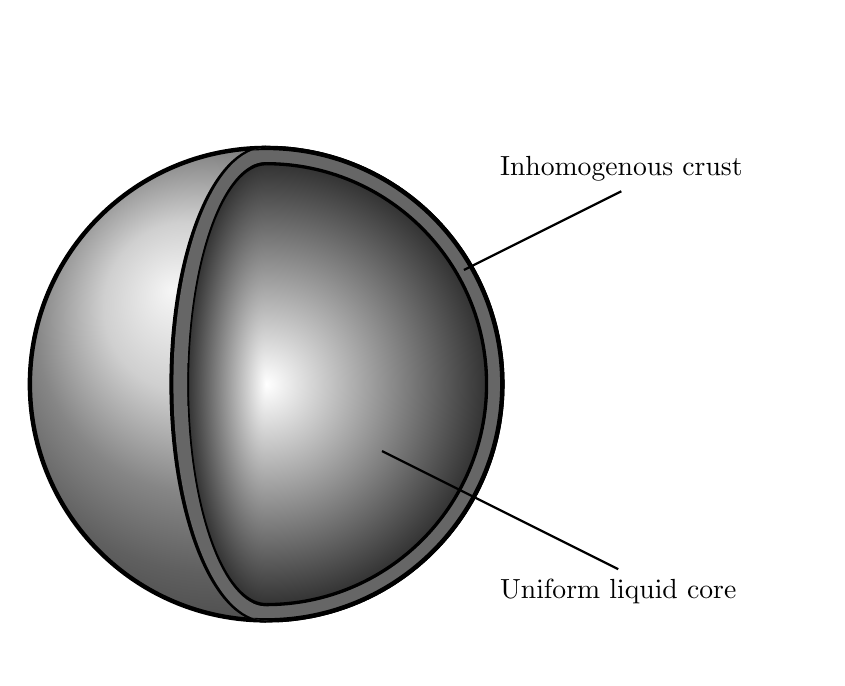
\begin{tikzpicture}[scale=1]
                \draw[ball color=gray!50,shading=ball, ultra thick, color=black] (0,0) circle (3cm);
                \draw[ultra thick] (0,3) arc (90:270:1.2cm and 3cm);
                \clip (0,-3) -- ++(7,-1) -- ++(0,8) -- ++(-7,-1) arc (90:270:1.177cm and 3cm) -- cycle;
                \draw[fill=gray!80!black, ultra thick] (0,0) circle (3cm); 
                \clip (0,-2.82) -- ++(7,-1) -- ++(0,7.64) -- ++(-7,-1) arc (90:270:1cm and 2.82cm) -- cycle;
                \shadedraw[draw=black, very thick,inner color=white, outer color=black!80] (0,0) circle (2.8cm);
                \draw[thick] (30:2.9cm) -- ++(2,1) node[above]{Inhomogenous crust};
                \draw[thick] (-30:1.7cm) -- ++(3,-1.5) node[below]{Uniform liquid core};
                \clip (0,2.82) arc (90:270:1.05cm and 2.82cm) -- cycle;
                \shadedraw[draw=black, very thick, inner color=white, outer color=black!80] (0,0) ellipse (1cm and 2.8cm);
        \end{tikzpicture}
        \caption{Simplified illustration of NS structure, where the baryon density decreases 
				(from white to dark gray) as we move outward from the center of NS.}
        \label{fig:NS_structure}
\end{figure} 

% \section{Tidal Deformation of Neutron Stars}%
% \label{sec:tidal_deformation_of_neutron_stars}
Given a realistic EoS of NS matter, the General Relativity not only explains 
the compact shape of NS in the hydrostatic equilibrium, but also predicts the interesting 
behavior of NS in a strong gravitational field. In particular, the shape of NS is 
tidally deformed to gain a nonzero quadrupole moment under the gravitational field 
formed by the mutual attraction of two coalescing NS's \cite{damour2009relativistic}. 
The first astronomical observation of a binary NS merger has been reported on August 17, 
2017, with the gravitational wave (\gls{GW}) signals detected by LIGO and Virgo laser 
interferometers \cite{abbott2017gw170817}, and the $\gamma$ ray burst (GRB) of very high intensity 
detected by the Fermi $\gamma$ ray space telescope \cite{abbott2017multi}. This exciting event 
is now widely referred to as GW170817, which opened a new era of the multimessenger 
astronomy. Following the GW signals from GW170817 \citep{abbott2017gw170817}, such signals have been detected two years later from a compact merger of two NS's dubbed as GW190425 
\citep{abbott2020gw190425}. The Bayesian analyses of these GW data resulted on the
empirical constraints for the tidal deformation of NS, as well as the gravitational 
mass $M$ and radius $R$ of NS \citep{abbott2018gw170817}. The \gls{NS} merger event 
is illustrated in Figure \ref{fig:NS_merger}, and one can see that
\begin{figure}[t]
        \centering
        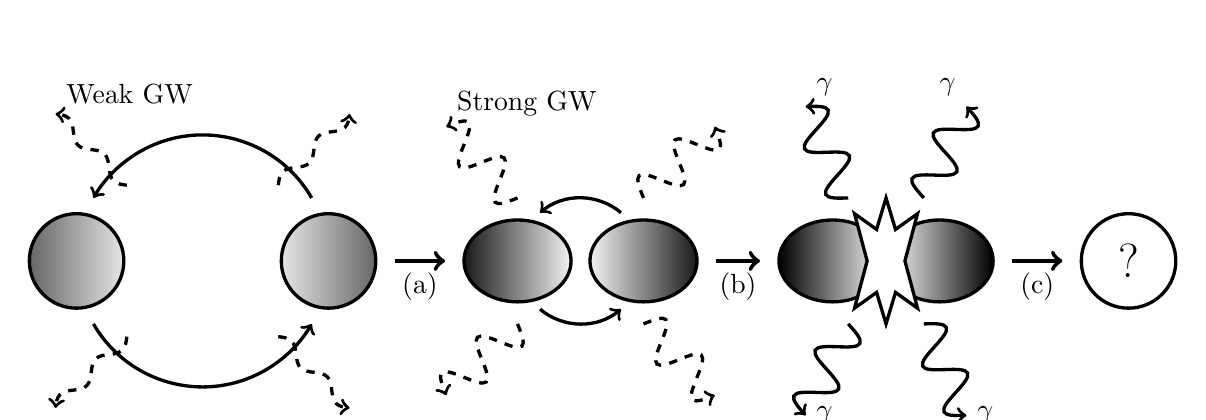
\begin{tikzpicture}[scale=0.8]
                \def\xl{-2};
                \def\xr{2};
                \def\r{0.75};
                \def\sep{3};
                \shadedraw[very thick, draw=black,left color=gray!80!black, right color=gray!20!white] (\xl,0) circle (\r cm);
                \shadedraw[very thick, draw=black,right color=gray!80!black, left color=gray!20!white] (\xr,0) circle (\r cm);
                \draw[->, very thick] (30:\xr cm) arc (30:150:\xr cm);
                \draw[->, very thick] (210:\xr cm) arc (210:330:\xr cm);
                \def\ang{-45};
                \draw[dashed, ->, very thick, cm={cos(\ang),-sin(\ang),sin(\ang),cos(\ang), (-\ang:1.7 cm)}] (0,0) sin (0.2,0.1) cos (0.4,0) sin (0.6,-0.1) cos (0.8,0) sin (1,0.1) cos (1.2,0) sin (1.4,-0.1) cos (1.6,0);
                \def\ang{-135};
                \draw[dashed, ->, very thick, cm={cos(\ang),-sin(\ang),sin(\ang),cos(\ang), (-\ang:1.7 cm)}] (0,0) sin (0.2,0.1) cos (0.4,0) sin (0.6,-0.1) cos (0.8,0) sin (1,0.1) cos (1.2,0) sin (1.4,-0.1) cos (1.6,0) node[above right]{Weak \gls{GW}};
                \def\ang{-225};
                \draw[dashed, ->, very thick, cm={cos(\ang),-sin(\ang),sin(\ang),cos(\ang), (-\ang:1.7 cm)}] (0,0) sin (0.2,0.1) cos (0.4,0) sin (0.6,-0.1) cos (0.8,0) sin (1,0.1) cos (1.2,0) sin (1.4,-0.1) cos (1.6,0);
                \def\ang{-315};
                \draw[dashed, ->, very thick, cm={cos(\ang),-sin(\ang),sin(\ang),cos(\ang), (-\ang:1.7 cm)}] (0,0) sin (0.2,0.1) cos (0.4,0) sin (0.6,-0.1) cos (0.8,0) sin (1,0.1) cos (1.2,0) sin (1.4,-0.1) cos (1.6,0);
                \draw[->, ultra thick] (\xr+\r+0.3,0) -- +(\sep-2*\r-0.7,0) node[pos=0.5,below]{(a)};

                \shadedraw[very thick, draw=black,left color=gray!20!black, right color=gray!10!white] (\xr+\sep,0) ellipse (0.85 cm and 0.65 cm);
                \shadedraw[very thick, draw=black,right color=gray!20!black, left color=gray!10!white] (\xr+\sep+2,0) ellipse (0.85 cm and 0.65 cm);
                \def\P{\xr+\sep+1};
                \def\R{1};
                \draw[->, very thick] (\P,0)+(50:\R cm) arc (50:130:\R cm);
                \draw[->, very thick] (\P,0)+(230:\R cm) arc (230:310:\R cm);
                \def\ang{-45};
                \draw[dashed, ->, very thick, cm={cos(\ang),-sin(\ang),sin(\ang),cos(\ang), (\P+1,1)}] (0,0) sin (0.2,0.3) cos (0.4,0) sin (0.6,-0.3) cos (0.8,0) sin (1,0.3) cos (1.2,0) sin (1.4,-0.3) cos (1.6,0);
                \def\ang{-135};
                \draw[dashed, ->, very thick, cm={cos(\ang),-sin(\ang),sin(\ang),cos(\ang), (\P-1,1)}] (0,0) sin (0.2,0.3) cos (0.4,0) sin (0.6,-0.3) cos (0.8,0) sin (1,0.3) cos (1.2,0) sin (1.4,-0.3) cos (1.6,0) node[above right]{Strong \gls{GW}};
                \def\ang{-225};
                \draw[dashed, ->, very thick, cm={cos(\ang),-sin(\ang),sin(\ang),cos(\ang), (\P-1,-1)}] (0,0) sin (0.2,0.3) cos (0.4,0) sin (0.6,-0.3) cos (0.8,0) sin (1,0.3) cos (1.2,0) sin (1.4,-0.3) cos (1.6,0);
                \def\ang{-315};
                \draw[dashed, ->, very thick, cm={cos(\ang),-sin(\ang),sin(\ang),cos(\ang), (\P+1,-1)}] (0,0) sin (0.2,0.3) cos (0.4,0) sin (0.6,-0.3) cos (0.8,0) sin (1,0.3) cos (1.2,0) sin (1.4,-0.3) cos (1.6,0);
                \draw[->, ultra thick] (\xr+\sep+2.85+0.3,0) -- +(\sep-2*0.85-0.6,0) node[pos=0.5,below]{(b)};

                \shadedraw[very thick, draw=black,left color=gray!0!black, right color=gray!0!white] (\xr+2*\sep+2,0) ellipse (0.85 cm and 0.65 cm);
                \shadedraw[very thick, draw=black,right color=gray!0!black, left color=gray!0!white] (\xr+2*\sep+3.7,0) ellipse (0.85 cm and 0.65 cm);
                \draw[->, ultra thick] (\xr+2*\sep+3.7+0.85+0.3,0) -- +(\sep-\r-0.85-0.6,0) node[pos=0.5,below]{(c)};
                \def\P{\xr+2*\sep+2.85};
                \draw[fill=white, very thick, shift={(\P,0)}] (0,1) -- (0.15,0.5) -- (0.5, 0.75) -- (0.3,0) -- (0.5,-0.75) -- (0.15,-0.5) -- (0,-1) -- (-0.15,-0.5) -- (-0.5,-0.75) -- (-0.3,0) -- (-0.5,0.75) -- (-0.15,0.5) -- cycle;
                \def\ang{-65};
                \draw[->, very thick, cm={cos(\ang),-sin(\ang),sin(\ang),cos(\ang), (\P+0.6,1)}] (0,0) sin (0.2,0.3) cos (0.4,0) sin (0.6,-0.3) cos (0.8,0) sin (1,0.3) cos (1.2,0) sin (1.4,-0.3) cos (1.6,0) node[above left]{$\gamma$};
                \def\ang{-115};
                \draw[->, very thick, cm={cos(\ang),-sin(\ang),sin(\ang),cos(\ang), (\P-0.6,1)}] (0,0) sin (0.2,0.3) cos (0.4,0) sin (0.6,-0.3) cos (0.8,0) sin (1,0.3) cos (1.2,0) sin (1.4,-0.3) cos (1.6,0) node[above right]{$\gamma$};
                \def\ang{-245};
                \draw[->, very thick, cm={cos(\ang),-sin(\ang),sin(\ang),cos(\ang), (\P-0.6,-1)}] (0,0) sin (0.2,0.3) cos (0.4,0) sin (0.6,-0.3) cos (0.8,0) sin (1,0.3) cos (1.2,0) sin (1.4,-0.3) cos (1.6,0) node[right]{$\gamma$};
                \def\ang{-295};
                \draw[->, very thick, cm={cos(\ang),-sin(\ang),sin(\ang),cos(\ang), (\P+0.6,-1)}] (0,0) sin (0.2,0.3) cos (0.4,0) sin (0.6,-0.3) cos (0.8,0) sin (1,0.3) cos (1.2,0) sin (1.4,-0.3) cos (1.6,0) node[right]{$\gamma$};

                \draw[very thick] (\xr+3.7+2*\sep+\sep,0) circle (\r cm) node{\LARGE ?};
        \end{tikzpicture}
        \caption{Illustration of the merger of a binary NS system. 
				(a) The two companion NS orbit about each others, while gradually losing 
				energy by emitting weak \gls{GW} and coming slowly closer with time. (b) As the 
				two \gls{NS} get closer, they accelerate and emit stronger \gls{GW} until (c) 
				merging with each other, which results in an extremely energetic explosion known 
				as \emph{kilonova}, an event associated
				with blue jets of \emph{gamma ray burst} (\gls{GRB}) of very high intensity. The end 
				product of the merger is either a small black hole (\gls{BH}) or a heavier \gls{NS}.}
        \label{fig:NS_merger}
\end{figure} 
gravitation exerted by each \gls{NS} tends to tidally ``stretch'' its companion while 
both orbiting spirally toward each other and dissipating energy through the emited 
\gls{GW}. As a result, the shape and mass-energy
distribution of \gls{NS} are tidally deformed from its supposedly spherical shape, 
leading to the nonzero multipole moments 
\citep{hinderer2008tidal,hinderer2010tidal,damour2009relativistic}. The tidal 
deformability of \gls{NS}, i.e., how strongly it deforms upon the impact of tidal field, 
is usually expressed in terms of the \emph{tidal Love numbers} $k_\ell$ of several orders 
$\ell$. In the present study, we evaluate the Love number of \gls{NS} 
up to the 4\textsuperscript{th} order, $\ell=2,3,4$ \citep{perot2021role}. It is naturally
to expect that the tidal Love number depends on the \gls{EoS} of NS matter, and this 
effect is discussed in Section \ref{chap:ns_prop}. Given very high baryon density in the
center of \gls{NS} (up to $6n_0$ where $n_0$ is the saturation density of normal NM ) 
the Love number of NS is of order $\sim 0.1$, while our Earth has that of $\sim 0.3$. 
In a recent study, the Love number has been predicted to be $\sim 0.002$ for spinning 
black holes with nearly infinite matter density inside \citep{le2021spinning}.

It is amazing that, like a charged sphere being electrically and magnetically deformed 
under a strong electromagnetic field, the tidal deformability of NS under the perturbation 
of spacetime can also be separated into the \emph{gravito-electric} (\gls{GE}) 
and \emph{gravito-magnetic} (\gls{GM}) components \citep{damour2009relativistic}. 
Namely, the tidal deformability (the Love number) of \gls{NS}  in the presence of tidal 
field can be characterized by the corresponding \gls{GE} ($k_\ell$) and \gls{GM} ($j_\ell$) 
components \citep{perot2021role}. This interesting result is presented in 
Section \ref{chap:ns_prop}.

\subsection*{Scope and Objectives}%
\label{sec:scope_and_objectives}

In summary, the study performed in this Thesis is focused on:
\begin{itemize}
        \item Inclusion of the spin polarization of baryons into the HF calculation
				of EoS of asymmetric NM \citep{tan2021equation},
        \item Dependence of the gravitational mass and radius of \gls{NS} on 
				different assumptions for the \gls{EoS} of NS matter,
        \item Sensitivity of \gls{GE} and \gls{GM} Love numbers of the tidal deformability 
				to the EoS of NS matter,
        \item Comparison of the calculated macroscopic properties of NS with the empirical
				astrophysical constraints inferred from the observed GW signals of the NS merger 
				\citep{abbott2018gw170817,xie2019bayesian}.
\end{itemize}


        \chapter{Hartree-Fock Calculation}
        \section{Nucleon-Nucleon Interaction}%
\label{sec:nucleon_nucleon_interaction}

Due to the lack of a exact theory to describe the nucleon-nucleon (\gls{NN}) interaction, a model need to be imposed and fit with experimental measurement or theoretical calculation results. Plus, for a system as massive as a \gls{NS}, deducing the \gls{EoS} using the \emph{ab initio} method, i.e. solving the Schr\"{o}dinger equation over all particles, is simply impossible, therefore an \emph{effective interaction} must be used \citep{greiner1996nuclear}. In this section, we only limit ourselves to two-body interaction, thus, the \gls{NN} potential can be expressed in the form of
\begin{equation}
        v = v(\bm{r}, \bm{r'}, \bm{p}, \bm{p'}, \bm{\sigma}, \bm{\sigma'}, \bm{\tau}, \bm{\tau'})
        \label{eff_interaction}
\end{equation}
where the primed and unprimed variables indicate the properties of 2 nucleons respectively, in which $\bm{r}$ is the particle's position, $\bm{p}$ is its momentum, $\bm{\sigma}$ is its intrinsic spin and $\bm{\tau}$ is its isospin.\par
The functional form of $v$ in \eqref{eff_interaction} cannot freely take any form but is constrained by many invariance requirements \citep{greiner1996nuclear}
\begin{itemize}
        \item \textbf{Translational invariance:} The \gls{NN} potential should only depend on the \emph{relative position} of the two particle but not their explicit positions, thus we can reduce \eqref{eff_interaction} to
                \begin{equation}
                        v = v(\bm{r}-\bm{r'},\bm{p},\bm{p'},\bm{\sigma},\bm{\sigma'},\bm{\tau},\bm{\tau'}) = v(\bm{r},\bm{p},\bm{p'},\bm{\sigma},\bm{\sigma'},\bm{\tau},\bm{\tau'})
                \end{equation}
                with at the last expression, we redefine $\bm{r}$ as the relative position vector.

        \item \textbf{Galilei invariance:} The potential should also be invariant under transformation between inertial frame of reference, which requires that only the relative momentum $\bm{p}-\bm{p'}$ is depended, i.e.
                \begin{equation}
                        v = v(\bm{r},\bm{p},\bm{\sigma},\bm{\sigma'},\bm{\tau},\bm{\tau'})
                        \label{eq2-3}
                \end{equation}
                where here we denote $\bm{p}$ as the relative momentum.

        \item \textbf{Rotational invariance:} The potential should be constructed such that the total angular momentum is zero.
                
        \item \textbf{Isospin invariance:} The \gls{NN} interaction potential needs to be invariant under rotation in isospin space, in other words, it can only depend on the isospin-independent terms and the terms with $\bm{\tau}\cdot\bm{\tau'}$. Therefore, we can split the potential into
                \begin{equation}
                        v = v_0 (\bm{r},\bm{p},\bm{\sigma},\bm{\sigma'}) + v_1 (\bm{r},\bm{p},\bm{\sigma},\bm{\sigma'}) \bm{\hat{\tau}}\cdot\bm{\hat{\tau}'}
                \end{equation}

        \item \textbf{Parity invariance:} The \gls{NN} interaction potential is also expected to be invariant under the action of parity operator, i.e. changing the sign of spatial coordinates
                \begin{equation}
                        v(\bm{r},\bm{p},\bm{\sigma},\bm{\sigma'},\bm{\tau},\bm{\tau'}) = v(-\bm{r},-\bm{p},\bm{\sigma},\bm{\sigma'},\bm{\tau},\bm{\tau'})
                \end{equation}

        \item \textbf{Time reversal invariance:} Finally, the interaction should stay the same after switching the time arrow direction
                \begin{equation}
                        v(\bm{r},\bm{p},\bm{\sigma},\bm{\sigma'},\bm{\tau},\bm{\tau'}) = v(\bm{r},-\bm{p},-\bm{\sigma},-\bm{\sigma'},\bm{\tau},\bm{\tau'})
                \end{equation}
\end{itemize}
Having the above considerations, developing further the M3Y-Paris interaction, which was used by the \gls{HF} study of \gls{NM} \citep{loan2011equation, tan2016mean, tan2020spin,tan2021equation} and the folding model study of \gls{NN} scattering \citep{khoa1997nuclear,khoa2000generalized},
\begin{equation}
        v = v_{00}(r) + v_{10}(r) \bm{\sigma}\cdot\bm{\sigma'} + v_{01}(r) \bm{\tau}\cdot\bm{\tau'} + v_{11}(r) (\bm{\sigma}\cdot\bm{\sigma'})(\bm{\tau}\cdot\bm{\tau'})
\end{equation}
by adding a density-dependent form factor to each term gives the CDM3Y$n$ interaction model
\begin{IEEEeqnarray*}{rCl}
        v(\rho,r) &=& F_{00}(\rho) v_{00}(r) + F_{10}(\rho) v_{10}(r) \bm{\sigma}\cdot\bm{\sigma'}\\
          &&\negmedspace{}+ F_{01}(\rho) v_{01}(r) \bm{\tau}\cdot\bm{\tau'} + F_{11}(\rho) v_{11}(r) (\bm{\sigma}\cdot\bm{\sigma'})(\bm{\tau}\cdot\bm{\tau'})\IEEEyesnumber
          \label{eq2-11}
\end{IEEEeqnarray*}  
where each radial term is the superposition of 3 Yukawa potentials
\begin{equation}
        v_{\sigma\tau}(r) = \sum^{3}_{k=1} Y_{\sigma\tau}(k) \frac{\exp(-\mu_k r)}{\mu_k r} 
\end{equation}
and the form factor $F_{\sigma\tau}(\rho)$ shared the functional form \citep{khoa1997nuclear,tan2020spin,tan2021equation,than2010ufr}
\begin{equation}
        F_{\sigma\tau}(\rho) = C_{\sigma\tau} [1 + \alpha_{\sigma\tau} \exp(-\beta_{\sigma\tau}\rho) + \gamma_{\sigma\tau}\rho]
\end{equation}
with parameters given in Table \ref{tab:cd}. The parameters of $F_{00}$ were adjusted to give the corresponding incompressibility $K$ of symmetric \gls{NM} at saturation density $\rho_0$ and the binding energy $E_0 \approx 15.8\; MeV$, while the 10 term is modified from \citep{than2010ufr} to reproduce $E_{sym}(\rho_0) \approx 30\;MeV$, $L\approx 50\;MeV$ and to be in agreement with the ab-initio results \citep{akmal1998equation,gandolfi2010microscopic} at higher density \citep{tan2021equation}. On the other hand, the spin-dependent terms, 10 and 11, are hereby included in the 5 models by fine tuning the parameters to yield the same result as the Brueckner-Hartree-Fock (\gls{BHF}) study of spin polarized \gls{NM} \citep{vidana2002equation} as in Figure \ref{fig:bhf}.

\begin{figure}[t]
        \centering
        \includegraphics[width=\textwidth]{fig/BHF_fit.eps}
        \caption{Energy per baryon $E/A$ of symmetric \gls{NM} by the 5 CDM3Y$n$ models compared to \gls{BHF} result \citep{vidana2002equation}. The diamond and square represent the \gls{BHF} result for $\Delta_n=-\Delta_p=\pm 1$ and $\Delta_n=\Delta_p=\pm 1$ respectively with $\Delta_\tau$ being the baryon spin polarity.}
        \label{fig:bhf}
\end{figure} 

\begin{table}[H]
        \centering
        \caption{CDM3Y$n$ interaction's parameters; the 00 and 01 terms are inherited from \citep{tan2021equation}, while the 10 and 11 parameters are added by fitting with \gls{BHF} result.}
        \label{tab:cd}
        \begin{tabular}{|C|C|C|C|C|C|C|}
                \hline
                \text{Interaction} & \sigma\tau & C_{\sigma\tau} & \alpha_{\sigma\tau} & \beta_{\sigma\tau} & \gamma_{\sigma\tau} & K\\
                                   & & & & (fm^3) & (fm^3) & (MeV)\\
                \hline
                \multirow{4}{*}{\text{CDM3Y3}} & 00 & 0.2985 & 3.4528 & 2.6388 & -1.5 &\multirow{4}{*}{217}\\
                                               & 01 & 0.2343 & 5.3336 & 6.4738 & 4.3172 &\\
                                               & 10 & 0.3890 & 3.5635 & -2.6717 & 20.3624 &\\
                                               & 11 & 0.8802 & 4.0433 & 12.3262 & 0.3662 &\\
                \hline
                \multirow{4}{*}{\text{CDM3Y4}} & 00 & 0.3052 & 3.2998 & 2.3180 & -2.0 &\multirow{4}{*}{228}\\
                                               & 01 & 0.2129 & 6.3581 & 7.0584 & 5.6091 &\\
                                               & 10 & 0.2593 & 6.0016 & -2.3377 & 18.8725 &\\
                                               & 11 & 0.8329 & 3.5941 & 9.2012 & 0.2690 &\\
                \hline
                \multirow{4}{*}{\text{CDM3Y5}} & 00 & 0.2728 & 3.7367 & 1.8294 & -3.0 &\multirow{4}{*}{241}\\
                                               & 01 & 0.2204 & 6.6146 & 7.9910 & 6.0040 &\\
                                               & 10 & 0.4106 & 5.6265 & -1.6698 & -1.9866 &\\
                                               & 11 & 0.6815 & 2.5833 & 5.1700 & 0.2578 &\\
                \hline
                \multirow{4}{*}{\text{CDM3Y6}} & 00 & 0.2658 & 3.8033 & 1.4099 & -4.0 &\multirow{4}{*}{252}\\
                                               & 01 & 0.2313 & 6.6865 & 8.6775 & 6.0182 &\\
                                               & 10 & 0.5186 & 9.9402 & 1.6698 & 2.9799 &\\
                                               & 11 & 0.6058 & 3.1947 & 4.4512 & 0.0822 &\\
                \hline
                \multirow{4}{*}{\text{CDM3Y8}} & 00 & 0.2658 & 3.8033 & 1.4099 & -4.3 &\multirow{4}{*}{257}\\
                                               & 01 & 0.2643 & 6.3836 & 9.8950 & 5.4249 &\\
                                               & 10 & 0.5997 & 9.1900 & 0.7514 & -4.7181 &\\
                                               & 11 & 0.3786 & 3.9435 & 2.7012 & 0.3512 &\\
                \hline
        \end{tabular}
\end{table}

\section{Equation of States of Nuclear Matter}%
\label{sec:equation_of_states_of_nuclear_matter}

In \gls{HF} formalism, the total \gls{HF} energy of the system can be expressed as
\begin{IEEEeqnarray*}{rCl}
        E_{HF} &=& \sum^{}_{\sigma\tau} \sum^{k_F^{\sigma\tau}}_{\bm{k}} \frac{\hbar^2 k^2}{2m_\tau} + \frac{1}{2} \sum^{}_{\bm{k}\sigma\tau} \sum^{}_{\bm{k'}\sigma'\tau'} \left[ \mel**{\bm{k}\sigma\tau,\bm{k'}\sigma'\tau'}{v^D}{\bm{k}\sigma\tau,\bm{k'}\sigma'\tau'} \right.\\
          && \left. \negmedspace{} + \mel**{\bm{k}\sigma\tau,\bm{k'}\sigma'\tau'}{v^{EX}}{\bm{k'}\sigma\tau,\bm{k}\sigma'\tau'} \right]\IEEEyesnumber
          \label{eqE}
\end{IEEEeqnarray*}  
where the single-particle wave function is plane wave
\begin{equation}
        \ket{\bm{k}\sigma\tau} = \frac{e^{i\bm{k}\cdot\bm{r}}}{ \sqrt{ \Omega}  } \chi_\sigma \chi_\tau
\end{equation}
$\Omega$ being the spatial volume of the system, $k_F^{\sigma\tau} = (6\pi^2 \rho_{\sigma\tau})^{1/3}$ is the Fermi momentum corresponding to spin $\sigma$ and isospin $\tau$, $v^{D(EX)}$ is the direct (exchange) part of the interaction determined from the singlet and triplet-even (odd) of the central \gls{NN} force. Adopting the same functional form of \eqref{eq2-11}, the direct and exchange interaction is written as
\begin{IEEEeqnarray*}{rCl}
        v^{D(EX)}(\rho_b,r) &=& F_{00}(\rho_b) v^{D(EX)}_{00}(r) + F_{10}(\rho_b) v^{D(EX)}_{10}(r) \bm{\sigma}\cdot\bm{\sigma'}\\
                          &&\negmedspace{}+ F_{01}(\rho_b) v^{D(EX)}_{01}(r) \bm{\tau}\cdot\bm{\tau'} + F_{11}(\rho_b) v^{D(EX)}_{11}(r) (\bm{\sigma}\cdot\bm{\sigma'})(\bm{\tau}\cdot\bm{\tau'})\IEEEyesnumber
                          \label{eqHF}
\end{IEEEeqnarray*}
and
\begin{IEEEeqnarray*}{rCl}
        v^{D(EX)}_{\sigma\tau}(r) &=& \sum^{3}_{k=1} Y^{D(EX)}_{\sigma\tau}(k) \frac{\exp(-\mu_k r)}{\mu_k r} \IEEEyesnumber
\end{IEEEeqnarray*}  
with the Yukawa strengths given in Table \ref{tab:yukawa} and the density-dependent form factor parameters are in Table \ref{tab:cd}. Note that in \eqref{eqHF}, $\rho_b$ denotes the \emph{baryon density}, this will be used in order to distinguish with the lepton density in the later section.

\begin{table}[H]
        \centering
        \caption{Yukawa strengths of the M3Y-Paris interaction \citep{tan2020spin,anantaraman1983effective}.}
        \label{tab:yukawa}
        \begin{tabular}{|C|C|C|C|C|C|C|C|C|C|}
                \hline
                k & \mu_k & Y^D_{00} & Y^D_{10} & Y^D_{01} & Y^D_{11} & Y^{EX}_{00} & Y^{EX}_{10} & Y^{EX}_{01} & Y^{EX}_{11}\\
                    & (fm^{-1}) & (MeV) & (MeV) & (MeV) & (MeV) & (MeV) & (MeV) & (MeV) & (MeV)\\
                \hline
                1 & 4.0& 11061.625 & 938.875 & 313.625 & -969.125 & -1524.25 & -3492.75 & -4118.0 & -2210.0\\
                2 & 2.5 & -2537.5 & -36.0 & 223.5 & 450.0 & -518.75 & 795.25 & 1054.75 & 568.75\\
                3 & 0.7072 & 0.0 & 0.0 & 0.0 & 3.4877 & -7.8474 & 2.6157 & 2.6157 & -0.8719\\
                \hline
        \end{tabular}
\end{table}
Multiply \eqref{eqE} with $\Omega^{-1}$, the energy density of the \gls{NM} is separated into the kinetic term $\varepsilon_{kin}$ and the potential terms $\varepsilon_{\sigma\tau}$, i.e.
\begin{equation}
        \varepsilon_{HF} = \frac{E_{HF}}{\Omega} = \varepsilon_{kin} + F_{00}(\rho_b) \varepsilon_{00} + F_{01}(\rho_b) \varepsilon_{01} + F_{10}(\rho_b) \varepsilon_{10} + F_{11}(\rho_b) \varepsilon_{11}
\end{equation}
The final expressions of each terms of the energy density are
\begin{IEEEeqnarray}{rCl}
        \varepsilon_{kin} &=& \frac{3}{10} \sum^{}_{\sigma\tau} \frac{\hbar^2 (k_F^{\sigma\tau})^2}{m_\tau} \rho_{\sigma\tau}\\
        \varepsilon_{00} &=& \frac{1}{2} \left[ \rho_b^2 J^D_{00} + \int {A^2_{00} v^{EX}_{00}(r)} \: d^3 r \right] \\
        \varepsilon_{10} &=& \frac{1}{2} \left[ \rho_b^2 J^D_{10} \left( \Delta_n \frac{1+\delta}{2} + \Delta_p \frac{1-\delta}{2} \right)^2 + \int {A^2_{10} v^{EX}_{10}(r)} \: d^3 r \right] \\
        \varepsilon_{01} &=& \frac{1}{2} \left[ \rho_b^2 J^D_{01}\delta^2 + \int {A^2_{01} v^{EX}_{01}(r)} \: d^3 r \right] \\
        \varepsilon_{11} &=& \frac{1}{2} \left[ \rho_b^2 J^D_{11} \left( \Delta_n \frac{1+\delta}{2} - \Delta_p \frac{1-\delta}{2} \right)^2 + \int {A^2_{11} v^{EX}_{11}(r)} \: d^3 r \right]
\end{IEEEeqnarray}  
where $\Delta_{\tau} = (\rho_{\uparrow \tau} - \rho_{\downarrow \tau})/\rho_{\tau}$ is the polarity of nucleon, $\delta = (\rho_n - \rho_p)/\rho_b$ is the asymmetry of \gls{NM}, $J^D_{\sigma\tau} = \int v^D_{\sigma\tau}(r)\: d^3 r$ is the volume integral of the direct interaction and
\begin{equation}
        \begin{array}{l}
                A_{00} = \rho_{\uparrow n} \hat{j_1}(k_F^{\uparrow n} r) + \rho_{\downarrow n} \hat{j_1}(k_F^{\downarrow n} r) + \rho_{\uparrow p} \hat{j_1}(k_F^{\uparrow p} r) + \rho_{\downarrow p} \hat{j_1}(k_F^{\downarrow p} r)\\[5pt]
                A_{10} = \rho_{\uparrow n} \hat{j_1}(k_F^{\uparrow n} r) - \rho_{\downarrow n} \hat{j_1}(k_F^{\downarrow n} r) + \rho_{\uparrow p} \hat{j_1}(k_F^{\uparrow p} r) - \rho_{\downarrow p} \hat{j_1}(k_F^{\downarrow p} r)\\[5pt]
                A_{01} = \rho_{\uparrow n} \hat{j_1}(k_F^{\uparrow n} r) + \rho_{\downarrow n} \hat{j_1}(k_F^{\downarrow n} r) - \rho_{\uparrow p} \hat{j_1}(k_F^{\uparrow p} r) - \rho_{\downarrow p} \hat{j_1}(k_F^{\downarrow p} r)\\[5pt]
                A_{11} = \rho_{\uparrow n} \hat{j_1}(k_F^{\uparrow n} r) - \rho_{\downarrow n} \hat{j_1}(k_F^{\downarrow n} r) - \rho_{\uparrow p} \hat{j_1}(k_F^{\uparrow p} r) + \rho_{\downarrow p} \hat{j_1}(k_F^{\downarrow p} r)
        \end{array}
\end{equation}
with $\hat{j}_1(x)=3j_1(x)/x$ and $j_1(x)$ being the 1\textsuperscript{st} order spherical Bessel function.

\section{\textbeta-Stable Nuclear Matter}%
\label{sec:textbeta_stable_nuclear_matter}

After the \gls{HF} calculation, we were able to obtain a numerical \gls{HF} energy density $\varepsilon(\rho_n,\rho_p,\Delta_n,\Delta_p)$. However, it is in fact impossible for a \gls{NS} to exist while consisting of purely nucleon. In order to compensate for this issue, leptons ($e^-$ and $\mu^-$) have to be introduced to the matter constituents and the $npe\mu$ matter has to satisfy the \emph{\textbeta-stable} condition \citep{glendenning2012compact}, i.e.
\begin{itemize}
        \item Charge balance
                \begin{equation}
                        \rho_p = \rho_e + \rho_\mu
                        \label{chargeEQ}
                \end{equation}
        \item Chemical potential balance
                \begin{equation}
                        \mu_n - \mu_p = \mu_e = \mu_\mu
                \end{equation}
                where $\mu_i = \pdv{\varepsilon}{\rho_i}$ ($i=n,p,e,\mu$) is the chemical potential of the $i$ particle.
\end{itemize}
The total energy density of the $npe\mu$ matter is thus
\begin{equation}
        \varepsilon = \varepsilon_{HF} + \rho_n m_n c^2 + \rho_p m_p c^2 + \varepsilon_e + \varepsilon_\mu 
\end{equation}
which leads to the nucleon chemical potential of the form
\begin{equation}
        \mu_\tau (\rho_n,\rho_p,\Delta_n,\Delta_p) = \frac{\partial \varepsilon}{\partial \rho_\tau}  = \frac{\partial \varepsilon_{HF}}{\partial \rho_\tau} + m_\tau c^2
\end{equation}
Let $\hat{\mu} = \mu_n - \mu_p$ be the leptons' chemical potential, \eqref{chargeEQ} is equivalent to\footnote{$\theta(x)$ is the Heaviside function, i.e. it returns $1$ for $x\geq 0$ and $0$ otherwise.}
\begin{equation}
        3\pi^2 (\hbar c)^3 \rho_p - \hat{\mu}^3 - \left[ \hat{\mu}^2 - (m_\mu c^2)^2 \right]^{3/2} \theta(\hat{\mu} - m_\mu c^2) = 0
\end{equation}
from which the proton fraction $x_p = \rho_p/\rho_b$ can be obtained as shown in Figure \ref{fig:xp}. Furthermore, under strong magnetic field like that of a magnetar, we can approximate $\Delta_n \approx -\Delta_p \approx \Delta$ and reduce the \gls{EoS} to depend on just the baryon polarity $\Delta$ alone, and the more baryon polarized, the stronger the magnetic field of the \gls{NS}.\par
For a fixed value of $\Delta$, we are able to obtain a density function of the form $\rho_n (\rho_b, \Delta)$ and $\rho_p (\rho_b, \Delta)$, which in turn gives the lepton chemical potential $\hat{\mu}(\rho_b,\Delta) = \hat{\mu}(\rho_n,\rho_p)$ On the other hand, the leptons' densities are then \cite{loan2011equation}
\begin{equation}
        \rho_e(\rho_b,\Delta) = \frac{ \hat{\mu}^3(\rho_b,\Delta)}{ 3\pi^2 (\hbar c)^3} \quad\text{and}\quad \rho_\mu(\rho_b,\Delta) = \frac{ \Big[\hat{\mu}^2(\rho_b,\Delta) - (m_\mu c^2)^2\Big]^{3/2}}{ 3\pi^2 (\hbar c)^3} \theta(\hat{\mu}(\rho_b,\Delta)-m_\mu c^2)
\end{equation} 
Consider the $e^-$ and $\mu^-$ to be systems of relativistic Fermi gas, then their respective energy densities and pressure contributions are ($l=e,\mu$) \citep{moustakidis2009equation}
\begin{equation}
        \varepsilon_l(\rho_b,\Delta) = \frac{ 2}{ (2\pi)^3} \int_{{0}}^{{[3\pi^2\rho_l(\rho_b,\Delta)]^{1/3}}} {\sqrt{\hbar^2 c^2 k^2 + m_l^2 c^4}} \: d^3{\mathbf{k}}
\end{equation} 
and
\begin{equation}
        P_l(\rho_b,\Delta) = \frac{ 1}{ 3} \frac{ 2}{ (2\pi)^3} \int_{{0}}^{{[3\pi^2 \rho_l(\rho_b,\Delta)]^{1/3}}} { \frac{ \hbar^2 c^2 k^2}{ \sqrt{\hbar^2 c^2 k^2 + m_l^2 c^4}} } \: d^3{\mathbf{k}}
\end{equation} 
Plus, from the \gls{HF} formalism with \gls{NM}, the baryon pressure is given by
\begin{equation}
        P_b = \rho_b^2 \pdv{(\varepsilon_{HF}/\rho_b)}{\rho_b}
\end{equation}
Finally, we obtain the total energy density dependence on baryon density as 
\begin{equation}
        \varepsilon(\rho_b,\Delta) = \varepsilon_{HF}(\rho_b,\Delta) + \rho_n(\rho_b,\Delta)m_n c^2 + \rho_p(\rho_b,\Delta)m_p c^2 + \varepsilon_e(\rho_b,\Delta) + \varepsilon_\mu(\rho_b,\Delta)
\end{equation}
and the total pressure of \gls{NS} matter
\begin{equation}
        P(\rho_b,\Delta) = P_b(\rho_b,\Delta) + P_e(\rho_b,\Delta) + P_\mu(\rho_b,\Delta)
\end{equation}
and this completes the \gls{EoS} of cold $\beta$-stable \gls{NS} matter (Figure \ref{fig:e} and \ref{fig:p}).


        \chapter{Neutron Star Properties}
        \section{Tolman-Oppenheimer-Volkoff Equation}%
\label{sec:tolman_oppenheimer_volkoff_equation}

In the framework of \gls{GR}, assume the \gls{NS} to be in a static, isotropic region of spacetime, the metric elements are then
\begin{equation}
        c^2 d\tau^2 = g_{\mu\nu} dx^\mu dx^\nu = e^{2\nu(r)}c^2 dt^2 - e^{2\lambda(r)} dr^2 - r^2 d\theta^2 - r^2\sin^2\theta d\phi^2
\end{equation}
Inside the \gls{NS}, we have \cite{glendenning2012compact} the energy-momentum tensor as
\begin{equation}
        T^{\mu\nu} = - Pg^{\mu\nu} + (P + \varepsilon) u^\mu u^\nu
\end{equation}
where $u^\mu = dx^\mu/d\tau$ is the local fluid 4-velocity. Solving the Einstein's field equation \cite{glendenning2012compact}
\begin{equation}
        G^{\mu\nu} = - \frac{8\pi G}{c^4} T^{\mu\nu} 
\end{equation}
gives the Tolman-Oppenheimer-Volkoff (\gls{TOV}) equation
\begin{IEEEeqnarray}{rCl}
        \frac{dP}{dr} &=& - \frac{G\varepsilon(P)m}{c^2 r^2} \left( 1+ \frac{P}{\varepsilon(P)} \right) \left( 1+ \frac{4\pi P r^3}{m c^2}  \right) \left( 1- \frac{2Gm}{c^2 r}  \right)^{-1}\\
        \frac{dm}{dr} &=& \frac{4\pi r^2\varepsilon(P)}{c^2}
\end{IEEEeqnarray}  
where $\varepsilon(P)$ can be obtained from the CDM3Y$n$ interaction calculated previously. Additional boundary conditions are
\begin{equation*}
        P(0)=P_c;\qquad P(R)=0;\qquad m(0)=0;\qquad m(R)=M
\end{equation*}
and by varying the center pressure $P_c$, a relation of the mass $M$ and radius $R$ of the \gls{NS} can be obtained.

\section{Gravito-electric and Gravito-magnetic Tidal Deformation}%
\label{sec:gravito_electric_and_gravito_magnetic_tidal_deformation}

Pertubing


        \clearpage
        \bibliographystyle{unsrt}
        \bibliography{ref}
\end{document}
